\documentclass[]{elsarticle} %review=doublespace preprint=single 5p=2 column
%%% Begin My package additions %%%%%%%%%%%%%%%%%%%
\usepackage[hyphens]{url}

  \journal{Homework 5 - A Wine Predictor} % Sets Journal name


\usepackage{lineno} % add
\providecommand{\tightlist}{%
  \setlength{\itemsep}{0pt}\setlength{\parskip}{0pt}}

\usepackage{graphicx}
%%%%%%%%%%%%%%%% end my additions to header

\usepackage[T1]{fontenc}
\usepackage{lmodern}
\usepackage{amssymb,amsmath}
\usepackage{ifxetex,ifluatex}
\usepackage{fixltx2e} % provides \textsubscript
% use upquote if available, for straight quotes in verbatim environments
\IfFileExists{upquote.sty}{\usepackage{upquote}}{}
\ifnum 0\ifxetex 1\fi\ifluatex 1\fi=0 % if pdftex
  \usepackage[utf8]{inputenc}
\else % if luatex or xelatex
  \usepackage{fontspec}
  \ifxetex
    \usepackage{xltxtra,xunicode}
  \fi
  \defaultfontfeatures{Mapping=tex-text,Scale=MatchLowercase}
  \newcommand{\euro}{€}
\fi
% use microtype if available
\IfFileExists{microtype.sty}{\usepackage{microtype}}{}
\bibliographystyle{elsarticle-harv}
\usepackage{longtable,booktabs,array}
\usepackage{calc} % for calculating minipage widths
% Correct order of tables after \paragraph or \subparagraph
\usepackage{etoolbox}
\makeatletter
\patchcmd\longtable{\par}{\if@noskipsec\mbox{}\fi\par}{}{}
\makeatother
% Allow footnotes in longtable head/foot
\IfFileExists{footnotehyper.sty}{\usepackage{footnotehyper}}{\usepackage{footnote}}
\makesavenoteenv{longtable}
\usepackage{graphicx}
\ifxetex
  \usepackage[setpagesize=false, % page size defined by xetex
              unicode=false, % unicode breaks when used with xetex
              xetex]{hyperref}
\else
  \usepackage[unicode=true]{hyperref}
\fi
\hypersetup{breaklinks=true,
            bookmarks=true,
            pdfauthor={},
            pdftitle={DS621-Homework 5},
            colorlinks=false,
            urlcolor=blue,
            linkcolor=magenta,
            pdfborder={0 0 0}}
\urlstyle{same}  % don't use monospace font for urls

\setcounter{secnumdepth}{0}
% Pandoc toggle for numbering sections (defaults to be off)
\setcounter{secnumdepth}{0}

% Pandoc citation processing

% Pandoc header
\usepackage{booktabs}
\usepackage{longtable}
\usepackage{array}
\usepackage{multirow}
\usepackage{wrapfig}
\usepackage{float}
\usepackage{colortbl}
\usepackage{pdflscape}
\usepackage{tabu}
\usepackage{threeparttable}
\usepackage{threeparttablex}
\usepackage[normalem]{ulem}
\usepackage{makecell}
\usepackage{xcolor}

\usepackage[nomarkers]{endfloat}

\begin{document}
\begin{frontmatter}

  \title{DS621-Homework 5}
    \author[Critical Thinking Group 2 - DS621]{George Cruz Deschamps}
   \ead{georg4re@gmail.com} 
    \author[Critical Thinking Group 2 - DS621]{Karim Hammoud}
   \ead{cunykarim@gmail.com} 
    \author[Critical Thinking Group 2 - DS621]{Maliat Islam}
   \ead{maliat.islam21@gmail.com} 
    \author[Critical Thinking Group 2 - DS621]{Matthew Lucich}
   \ead{matt.lucich@gmail.com} 
    \author[Critical Thinking Group 2 - DS621]{Gabriella Martinez}
   \ead{gpmmrtzz@gmail.com} 
    \author[Critical Thinking Group 2 - DS621]{Ken Popkin}
   \ead{krpopkin@gmail.com} 
      
  \begin{abstract}
  A large wine manufacturer is studying the data in order to predict the
  number of wine cases ordered based upon the wine characteristics. If the
  wine manufacturer can predict the number of cases, then that
  manufacturer will be able to adjust their wine offering to maximize
  sales. Our objective is to build a count regression model to predict the
  number of cases of wine that will be sold given certain properties of
  the wine.
  \end{abstract}
  
 \end{frontmatter}

\newpage

\hypertarget{data-exploration}{%
\section{Data Exploration}\label{data-exploration}}

Let's take an initial look at our data. The summary looks like this:

\begin{longtable}[]{@{}ll@{}}
\toprule
\textbf{Characteristic} & \textbf{N = 12,795}\tabularnewline
\midrule
\endhead
TARGET &\tabularnewline
0 & 2,734 / 12,795 (21\%)\tabularnewline
1 & 244 / 12,795 (1.9\%)\tabularnewline
2 & 1,091 / 12,795 (8.5\%)\tabularnewline
3 & 2,611 / 12,795 (20\%)\tabularnewline
4 & 3,177 / 12,795 (25\%)\tabularnewline
5 & 2,014 / 12,795 (16\%)\tabularnewline
6 & 765 / 12,795 (6.0\%)\tabularnewline
7 & 142 / 12,795 (1.1\%)\tabularnewline
8 & 17 / 12,795 (0.1\%)\tabularnewline
FixedAcidity & 7.08 (6.32)\tabularnewline
VolatileAcidity & 0.32 (0.78)\tabularnewline
CitricAcid & 0.31 (0.86)\tabularnewline
ResidualSugar & 5.42 (33.75)\tabularnewline
(Missing) & 616\tabularnewline
Chlorides & 0.05 (0.32)\tabularnewline
(Missing) & 638\tabularnewline
FreeSulfurDioxide & 30.85 (148.71)\tabularnewline
(Missing) & 647\tabularnewline
TotalSulfurDioxide & 120.71 (231.91)\tabularnewline
(Missing) & 682\tabularnewline
Density & 0.99 (0.03)\tabularnewline
pH & 3.21 (0.68)\tabularnewline
(Missing) & 395\tabularnewline
Sulphates & 0.53 (0.93)\tabularnewline
(Missing) & 1,210\tabularnewline
Alcohol & 10.49 (3.73)\tabularnewline
(Missing) & 653\tabularnewline
LabelAppeal &\tabularnewline
-2 & 504 / 12,795 (3.9\%)\tabularnewline
-1 & 3,136 / 12,795 (25\%)\tabularnewline
0 & 5,617 / 12,795 (44\%)\tabularnewline
1 & 3,048 / 12,795 (24\%)\tabularnewline
2 & 490 / 12,795 (3.8\%)\tabularnewline
AcidIndex & 7.77 (1.32)\tabularnewline
STARS &\tabularnewline
1 & 3,042 / 9,436 (32\%)\tabularnewline
2 & 3,570 / 9,436 (38\%)\tabularnewline
3 & 2,212 / 9,436 (23\%)\tabularnewline
4 & 612 / 9,436 (6.5\%)\tabularnewline
(Missing) & 3,359\tabularnewline
\bottomrule
\end{longtable}

Our dataset consists of 15 variables and 12,795 observations. There are
some missing values on ResidualSugar, Chlorides, FreeSulfurDioxide,
TotalSulfurDioxide, pH, Sulphates, Alcohol, and STARS variables. TARGET
is our response variable. LabelAppeal, AcidIndex, and STARS are discrete
variables and the rest are continuous.

\begin{verbatim}
## Dataset for this assignment is 12795 instances and 16 features
\end{verbatim}

\textbf{Missing Values Count:}

\begin{longtable}[]{@{}lr@{}}
\toprule
Variable & Missing\tabularnewline
\midrule
\endhead
ResidualSugar & 616\tabularnewline
Chlorides & 638\tabularnewline
FreeSulfurDioxide & 647\tabularnewline
TotalSulfurDioxide & 682\tabularnewline
pH & 395\tabularnewline
Sulphates & 1210\tabularnewline
Alcohol & 653\tabularnewline
STARS & 3359\tabularnewline
\bottomrule
\end{longtable}

\begin{center}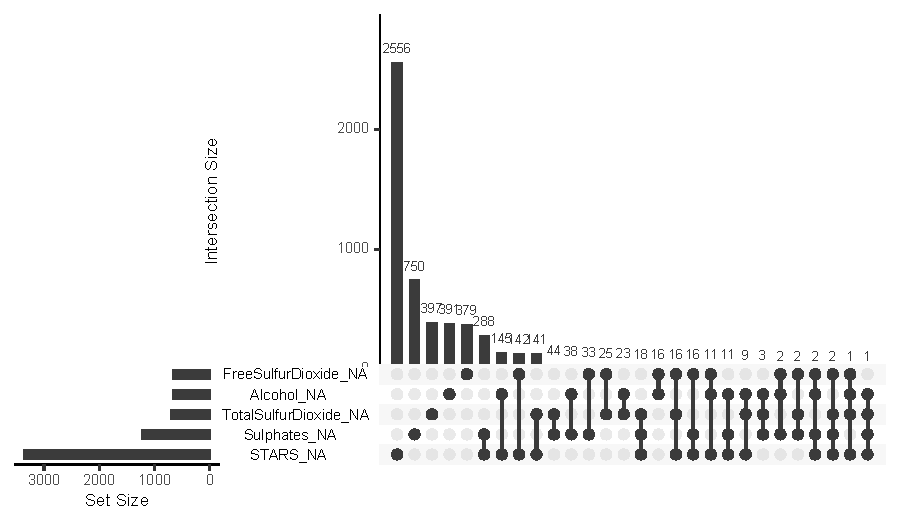
\includegraphics{paper_files/figure-latex/unnamed-chunk-5-1} \end{center}

\newpage

\hypertarget{data-visualization}{%
\subsubsection{Data Visualization}\label{data-visualization}}

In the box plots below, we can see \texttt{TotalSulfurDioxide},
\texttt{FreeSulfurDioxide}, and \texttt{ResidualSugar} variables have
large ranges compared to the other variables. We can tell a high number
of variables have outliers. Almost all of the variables are centered
around zero and at least four of the variables have negative values.

\begin{center}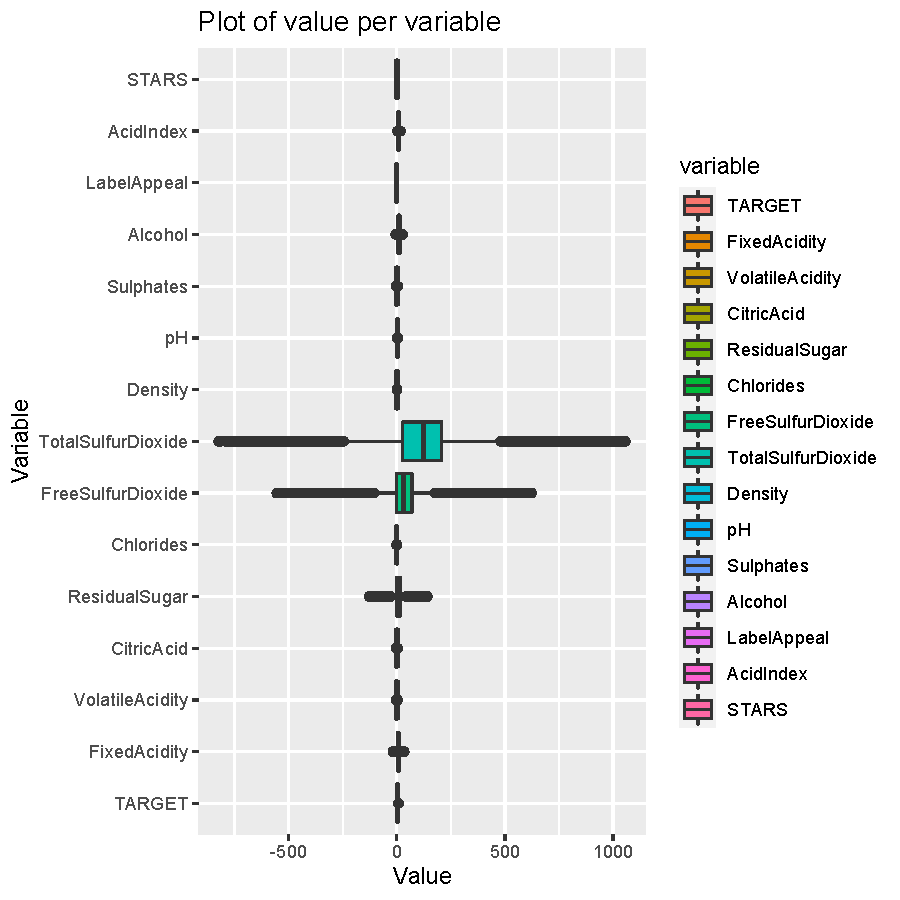
\includegraphics{paper_files/figure-latex/unnamed-chunk-6-1} \end{center}

\begin{center}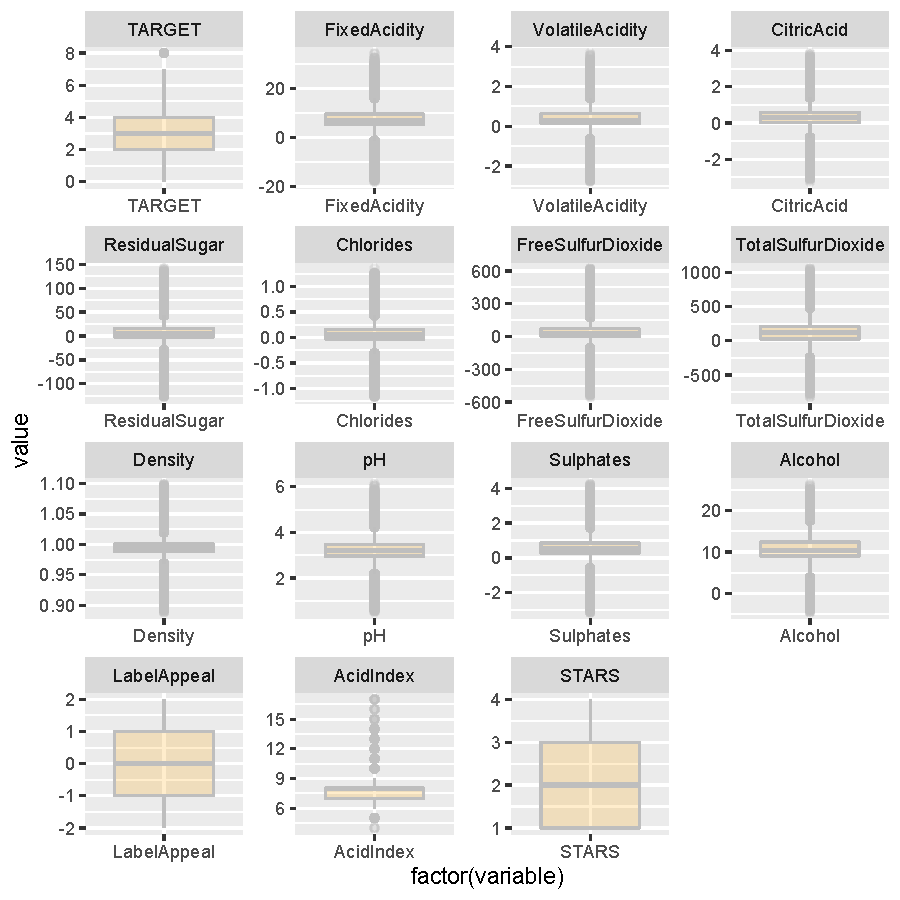
\includegraphics{paper_files/figure-latex/unnamed-chunk-7-1} \end{center}

\newpage

\hypertarget{data-correlations}{%
\subsubsection{Data correlations}\label{data-correlations}}

We also take a look at the correlation between the variables.

\begin{longtable}[]{@{}llr@{}}
\toprule
& colnames\_vector & res\_vector\tabularnewline
\midrule
\endhead
2 & STARS & 0.5588\tabularnewline
3 & LabelAppeal & 0.3565\tabularnewline
4 & Alcohol & 0.0621\tabularnewline
5 & TotalSulfurDioxide & 0.0515\tabularnewline
6 & FreeSulfurDioxide & 0.0438\tabularnewline
7 & ResidualSugar & 0.0165\tabularnewline
8 & CitricAcid & 0.0087\tabularnewline
9 & INDEX & 0.0013\tabularnewline
10 & pH & -0.0094\tabularnewline
11 & Density & -0.0355\tabularnewline
12 & Chlorides & -0.0383\tabularnewline
13 & Sulphates & -0.0388\tabularnewline
14 & FixedAcidity & -0.0490\tabularnewline
15 & VolatileAcidity & -0.0888\tabularnewline
16 & AcidIndex & -0.2460\tabularnewline
\bottomrule
\end{longtable}

\begin{center}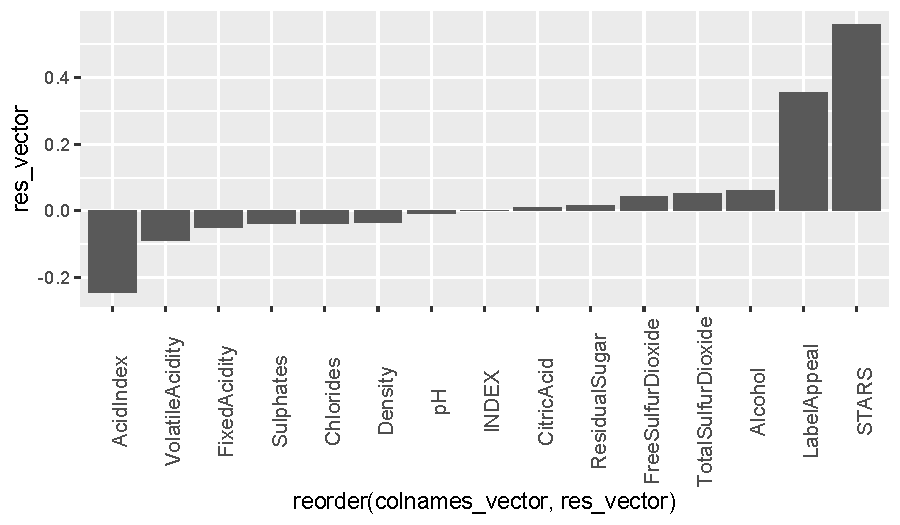
\includegraphics{paper_files/figure-latex/unnamed-chunk-9-1} \end{center}

In the above correlation table and plot \texttt{STARS} and
\texttt{LabelAppeal} appear to be most positively correlated variables
with the response variable. We can also see some mild negative
correlation between the response variable and \texttt{AcidIndex}.

\newpage

\hypertarget{data-manipulation}{%
\section{Data Manipulation}\label{data-manipulation}}

\hypertarget{recommendations}{%
\subsubsection{Recommendations}\label{recommendations}}

\begin{enumerate}
\def\labelenumi{\arabic{enumi}.}
\tightlist
\item
  \textbf{Address Missing Values} The features below have missing
  values. Recommendation to address this for each feature is:\\
\end{enumerate}

\begin{enumerate}
\def\labelenumi{\alph{enumi}.}
\tightlist
\item
  \textbf{Residual Sugar (616):} replace missing values with mean
  because normal dist, corr w/target is 0, \& most target values have a
  similar mean. 
\item
  \textbf{Chlorides (638):} same as Residual Sugar (replace with mean)
\item
  \textbf{Free Sulfur Dioxide (647):} same as Residual Sugar 
\item
  \textbf{Total Sulfur Dioxide (682):} same as Residual Sugar
  (considered using median, but mean is 120 and median is 123, so not
  much difference) 
\item
  \textbf{PH (395):} same as Residual Sugar 
\item
  \textbf{Sulphates (1210):} same as Residual Sugar\\
\item
  \textbf{Alcohol (653):} replace missing values with mean. Correlation
  is higher on this feature at around 12\% 
\item
  \textbf{STARS (3359):} values are 1 to 4. replace missing values with
  a 0 to indicate no ranking provided. 
\end{enumerate}

\begin{enumerate}
\def\labelenumi{\arabic{enumi}.}
\setcounter{enumi}{1}
\tightlist
\item
  \textbf{Apply Scalar} Max values are wide ranging across the features.
  For example, \texttt{Volatile\ Acidity}'s max value is 4 and
  \texttt{SulfurDioxide\textquotesingle{}s} max value is 1038. Recommend
  applying StandardScalar prior to modeling.
\end{enumerate}

\newpage

\hypertarget{data-modeling}{%
\section{Data Modeling}\label{data-modeling}}

\hypertarget{poisson-model-with-inputted-missing-values}{%
\subsubsection{Poisson model (with inputted missing
values)}\label{poisson-model-with-inputted-missing-values}}

\begin{longtable}[]{@{}llll@{}}
\toprule
\textbf{Characteristic} & \textbf{IRR} & \textbf{95\% CI} &
\textbf{p-value}\tabularnewline
\midrule
\endhead
FixedAcidity & 1.00 & 1.00, 1.00 & 0.7\tabularnewline
VolatileAcidity & 0.97 & 0.95, 0.98 & \textless0.001\tabularnewline
CitricAcid & 1.01 & 1.00, 1.02 & 0.2\tabularnewline
ResidualSugar & 1.00 & 1.00, 1.00 & 0.7\tabularnewline
Chlorides & 0.96 & 0.93, 0.99 & 0.012\tabularnewline
FreeSulfurDioxide & 1.00 & 1.00, 1.00 & \textless0.001\tabularnewline
TotalSulfurDioxide & 1.00 & 1.00, 1.00 & \textless0.001\tabularnewline
Density & 0.75 & 0.52, 1.10 & 0.14\tabularnewline
pH & 0.98 & 0.97, 1.00 & 0.040\tabularnewline
Sulphates & 0.99 & 0.98, 1.00 & 0.027\tabularnewline
Alcohol & 1.00 & 1.00, 1.00 & 0.12\tabularnewline
LabelAppeal & 1.14 & 1.13, 1.16 & \textless0.001\tabularnewline
AcidIndex & 0.92 & 0.91, 0.92 & \textless0.001\tabularnewline
STARS & 1.37 & 1.35, 1.38 & \textless0.001\tabularnewline
\bottomrule
\end{longtable}

\hypertarget{poisson-model-with-significant-variables.}{%
\subsubsection{Poisson model with significant
variables.}\label{poisson-model-with-significant-variables.}}

\begin{longtable}[]{@{}llll@{}}
\toprule
\textbf{Characteristic} & \textbf{IRR} & \textbf{95\% CI} &
\textbf{p-value}\tabularnewline
\midrule
\endhead
VolatileAcidity & 0.96 & 0.95, 0.98 & \textless0.001\tabularnewline
AcidIndex & 0.92 & 0.91, 0.93 & \textless0.001\tabularnewline
STARS & 1.41 & 1.40, 1.42 & \textless0.001\tabularnewline
\bottomrule
\end{longtable}

\hypertarget{negative-binomial-with-inputted-missing-values}{%
\subsubsection{Negative Binomial (with inputted missing
values)}\label{negative-binomial-with-inputted-missing-values}}

\begin{longtable}[]{@{}llll@{}}
\toprule
\textbf{Characteristic} & \textbf{IRR} & \textbf{95\% CI} &
\textbf{p-value}\tabularnewline
\midrule
\endhead
INDEX & 1.00 & 1.00, 1.00 & 0.7\tabularnewline
FixedAcidity & 1.00 & 1.00, 1.00 & 0.7\tabularnewline
VolatileAcidity & 0.97 & 0.95, 0.98 & \textless0.001\tabularnewline
CitricAcid & 1.01 & 1.00, 1.02 & 0.2\tabularnewline
ResidualSugar & 1.00 & 1.00, 1.00 & 0.7\tabularnewline
Chlorides & 0.96 & 0.93, 0.99 & 0.012\tabularnewline
FreeSulfurDioxide & 1.00 & 1.00, 1.00 & \textless0.001\tabularnewline
TotalSulfurDioxide & 1.00 & 1.00, 1.00 & \textless0.001\tabularnewline
Density & 0.75 & 0.52, 1.10 & 0.14\tabularnewline
pH & 0.98 & 0.97, 1.00 & 0.040\tabularnewline
Sulphates & 0.99 & 0.98, 1.00 & 0.028\tabularnewline
Alcohol & 1.00 & 1.00, 1.00 & 0.12\tabularnewline
LabelAppeal & 1.14 & 1.13, 1.16 & \textless0.001\tabularnewline
AcidIndex & 0.92 & 0.91, 0.92 & \textless0.001\tabularnewline
STARS & 1.37 & 1.35, 1.38 & \textless0.001\tabularnewline
\bottomrule
\end{longtable}

\hypertarget{negative-binomial-model-with-significant-values.}{%
\subsubsection{Negative binomial model with significant
values.}\label{negative-binomial-model-with-significant-values.}}

\begin{longtable}[]{@{}llll@{}}
\toprule
\textbf{Characteristic} & \textbf{IRR} & \textbf{95\% CI} &
\textbf{p-value}\tabularnewline
\midrule
\endhead
VolatileAcidity & 0.97 & 0.96, 0.98 & \textless0.001\tabularnewline
FreeSulfurDioxide & 1.00 & 1.00, 1.00 & 0.011\tabularnewline
TotalSulfurDioxide & 1.00 & 1.00, 1.00 & 0.001\tabularnewline
Alcohol & 1.00 & 1.00, 1.01 & 0.002\tabularnewline
as.factor(LabelAppeal) & & &\tabularnewline
-2 & & &\tabularnewline
-1 & 1.27 & 1.18, 1.37 & \textless0.001\tabularnewline
0 & 1.54 & 1.43, 1.65 & \textless0.001\tabularnewline
1 & 1.76 & 1.63, 1.89 & \textless0.001\tabularnewline
2 & 2.01 & 1.85, 2.19 & \textless0.001\tabularnewline
as.factor(AcidIndex) & & &\tabularnewline
4 & & &\tabularnewline
5 & 0.86 & 0.48, 1.73 & 0.6\tabularnewline
6 & 0.90 & 0.51, 1.79 & 0.7\tabularnewline
7 & 0.87 & 0.49, 1.73 & 0.7\tabularnewline
8 & 0.84 & 0.48, 1.68 & 0.6\tabularnewline
9 & 0.75 & 0.43, 1.50 & 0.4\tabularnewline
10 & 0.64 & 0.36, 1.29 & 0.2\tabularnewline
11 & 0.45 & 0.25, 0.90 & 0.012\tabularnewline
12 & 0.44 & 0.24, 0.89 & 0.012\tabularnewline
13 & 0.52 & 0.29, 1.06 & 0.047\tabularnewline
14 & 0.47 & 0.25, 0.98 & 0.028\tabularnewline
15 & 0.74 & 0.34, 1.69 & 0.5\tabularnewline
16 & 0.39 & 0.12, 1.09 & 0.082\tabularnewline
17 & 0.30 & 0.09, 0.84 & 0.028\tabularnewline
as.factor(STARS) & & &\tabularnewline
0 & & &\tabularnewline
1 & 2.13 & 2.05, 2.21 & \textless0.001\tabularnewline
2 & 2.93 & 2.83, 3.04 & \textless0.001\tabularnewline
3 & 3.30 & 3.18, 3.43 & \textless0.001\tabularnewline
4 & 3.72 & 3.55, 3.90 & \textless0.001\tabularnewline
\bottomrule
\end{longtable}

\hypertarget{linear-model-with-scaled-significant-data.}{%
\subsubsection{Linear Model with scaled significant
data.}\label{linear-model-with-scaled-significant-data.}}

\begin{longtable}[]{@{}llll@{}}
\toprule
\textbf{Characteristic} & \textbf{Beta} & \textbf{95\% CI} &
\textbf{p-value}\tabularnewline
\midrule
\endhead
VolatileAcidity & -0.04 & -0.05, -0.03 & \textless0.001\tabularnewline
FreeSulfurDioxide & 0.02 & 0.01, 0.03 & \textless0.001\tabularnewline
TotalSulfurDioxide & 0.03 & 0.01, 0.04 & \textless0.001\tabularnewline
Alcohol & 0.03 & 0.01, 0.04 & \textless0.001\tabularnewline
as.factor(LabelAppeal) & & &\tabularnewline
-2.23426998624856 & & &\tabularnewline
-1.11204793733397 & 0.19 & 0.13, 0.25 & \textless0.001\tabularnewline
0.0101741115806247 & 0.43 & 0.37, 0.50 & \textless0.001\tabularnewline
1.13239616049522 & 0.68 & 0.61, 0.74 & \textless0.001\tabularnewline
2.25461820940981 & 1.0 & 0.89, 1.1 & \textless0.001\tabularnewline
as.factor(AcidIndex) & & &\tabularnewline
-2.84964768611181 & & &\tabularnewline
-2.09431867252628 & -0.16 & -0.94, 0.62 & 0.7\tabularnewline
-1.33898965894075 & -0.10 & -0.87, 0.66 & 0.8\tabularnewline
-0.583660645355226 & -0.15 & -0.92, 0.61 & 0.7\tabularnewline
0.171668368230302 & -0.21 & -1.0, 0.56 & 0.6\tabularnewline
0.926997381815829 & -0.37 & -1.1, 0.40 & 0.3\tabularnewline
1.68232639540136 & -0.53 & -1.3, 0.24 & 0.2\tabularnewline
2.43765540898688 & -0.78 & -1.5, -0.01 & 0.049\tabularnewline
3.19298442257241 & -0.78 & -1.6, -0.01 & 0.047\tabularnewline
3.94831343615794 & -0.79 & -1.6, -0.01 & 0.048\tabularnewline
4.70364244974347 & -0.71 & -1.5, 0.08 & 0.077\tabularnewline
5.45897146332899 & -0.32 & -1.2, 0.58 & 0.5\tabularnewline
6.21430047691452 & -0.89 & -1.9, 0.08 & 0.073\tabularnewline
6.96962949050005 & -1.0 & -1.9, -0.07 & 0.035\tabularnewline
as.factor(STARS) & & &\tabularnewline
-1.26902307229896 & & &\tabularnewline
-0.42623524866846 & 0.70 & 0.67, 0.74 & \textless0.001\tabularnewline
0.416552574962037 & 1.2 & 1.2, 1.3 & \textless0.001\tabularnewline
1.25934039859254 & 1.5 & 1.5, 1.6 & \textless0.001\tabularnewline
2.10212822222303 & 1.9 & 1.8, 1.9 & \textless0.001\tabularnewline
\bottomrule
\end{longtable}

\hypertarget{linear-model-without-the-scaled-value.}{%
\subsubsection{Linear model without the scaled
value.}\label{linear-model-without-the-scaled-value.}}

\begin{longtable}[]{@{}llll@{}}
\toprule
\textbf{Characteristic} & \textbf{Beta} & \textbf{95\% CI} &
\textbf{p-value}\tabularnewline
\midrule
\endhead
INDEX & 0.00 & 0.00, 0.00 & 0.7\tabularnewline
FixedAcidity & 0.00 & 0.00, 0.00 & \textgreater0.9\tabularnewline
VolatileAcidity & -0.10 & -0.13, -0.07 & \textless0.001\tabularnewline
CitricAcid & 0.02 & -0.01, 0.05 & 0.13\tabularnewline
ResidualSugar & 0.00 & 0.00, 0.00 & 0.6\tabularnewline
Chlorides & -0.12 & -0.20, -0.05 & \textless0.001\tabularnewline
FreeSulfurDioxide & 0.00 & 0.00, 0.00 & \textless0.001\tabularnewline
TotalSulfurDioxide & 0.00 & 0.00, 0.00 & \textless0.001\tabularnewline
Density & -0.80 & -1.7, 0.07 & 0.071\tabularnewline
pH & -0.03 & -0.07, 0.00 & 0.049\tabularnewline
Sulphates & -0.03 & -0.06, -0.01 & 0.013\tabularnewline
Alcohol & 0.01 & 0.00, 0.02 & \textless0.001\tabularnewline
LabelAppeal & 0.43 & 0.41, 0.46 & \textless0.001\tabularnewline
AcidIndex & -0.21 & -0.23, -0.19 & \textless0.001\tabularnewline
STARS & 1.0 & 1.0, 1.0 & \textless0.001\tabularnewline
\bottomrule
\end{longtable}

\hypertarget{zero-inflation-with-inputted-missing-values.}{%
\subsubsection{Zero inflation with inputted Missing
Values.}\label{zero-inflation-with-inputted-missing-values.}}

\begin{verbatim}
## 
## Call:
## zeroinfl(formula = TARGET ~ . | STARS, data = data_mv, dist = "negbin")
## 
## Pearson residuals:
##      Min       1Q   Median       3Q      Max 
## -2.31701 -0.53688  0.01918  0.40829  2.89146 
## 
## Count model coefficients (negbin with log link):
##                      Estimate Std. Error z value Pr(>|z|)
## (Intercept)         1.543e+00         NA      NA       NA
## INDEX               1.809e-07         NA      NA       NA
## FixedAcidity        3.013e-04         NA      NA       NA
## VolatileAcidity    -1.499e-02         NA      NA       NA
## CitricAcid          1.243e-03         NA      NA       NA
## ResidualSugar      -4.969e-05         NA      NA       NA
## Chlorides          -2.335e-02         NA      NA       NA
## FreeSulfurDioxide   3.718e-05         NA      NA       NA
## TotalSulfurDioxide -2.958e-06         NA      NA       NA
## Density            -2.732e-01         NA      NA       NA
## pH                  2.922e-03         NA      NA       NA
## Sulphates          -1.947e-03         NA      NA       NA
## Alcohol             6.542e-03         NA      NA       NA
## LabelAppeal         2.240e-01         NA      NA       NA
## AcidIndex          -3.130e-02         NA      NA       NA
## STARS               1.007e-01         NA      NA       NA
## Log(theta)          1.797e+01         NA      NA       NA
## 
## Zero-inflation model coefficients (binomial with logit link):
##             Estimate Std. Error z value Pr(>|z|)
## (Intercept)   0.3804         NA      NA       NA
## STARS        -2.2238         NA      NA       NA
## 
## Theta = 63997386.9979 
## Number of iterations in BFGS optimization: 23 
## Log-likelihood: -2.083e+04 on 19 Df
\end{verbatim}

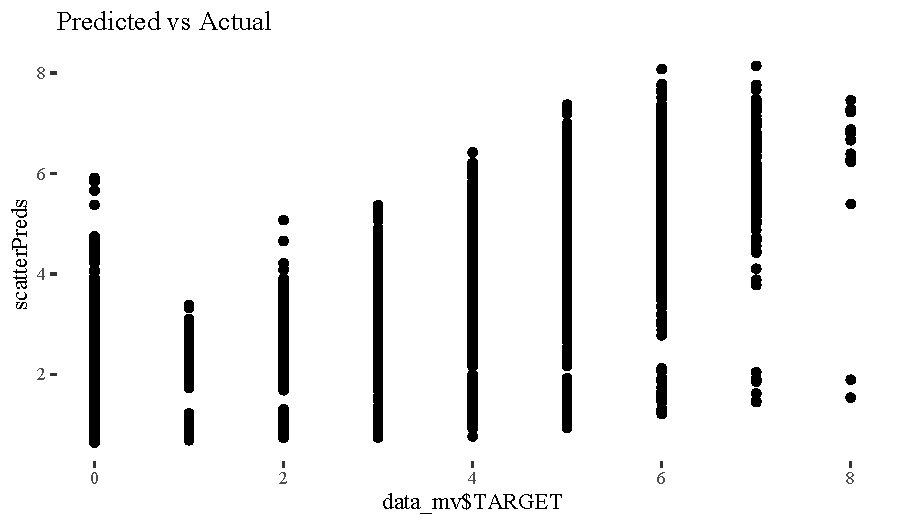
\includegraphics{paper_files/figure-latex/unnamed-chunk-29-1.pdf}

The scaled dataset was transformed into absolute value dataset as
Poisson and Negative Binomial were unable to work with negative data.

\hypertarget{absolute-value-poisson}{%
\subsubsection{Absolute Value Poisson}\label{absolute-value-poisson}}

\begin{verbatim}
## 
## Call:
## glm(formula = TARGET ~ ., family = poisson, data = absdata)
## 
## Deviance Residuals: 
##     Min       1Q   Median       3Q      Max  
## -1.8550  -0.5038  -0.0667   0.4644   1.5768  
## 
## Coefficients:
##                     Estimate Std. Error z value Pr(>|z|)    
## (Intercept)        -0.920316   0.041520 -22.166   <2e-16 ***
## INDEX               0.012386   0.019653   0.630    0.529    
## FixedAcidity        0.001218   0.013445   0.091    0.928    
## VolatileAcidity     0.017113   0.013199   1.296    0.195    
## CitricAcid          0.002713   0.013125   0.207    0.836    
## ResidualSugar      -0.004542   0.013001  -0.349    0.727    
## Chlorides           0.001761   0.012668   0.139    0.889    
## FreeSulfurDioxide  -0.002295   0.012879  -0.178    0.859    
## TotalSulfurDioxide  0.003254   0.013308   0.245    0.807    
## Density             0.008868   0.012986   0.683    0.495    
## pH                  0.004886   0.013442   0.363    0.716    
## Sulphates           0.013197   0.012680   1.041    0.298    
## Alcohol            -0.007084   0.013916  -0.509    0.611    
## LabelAppeal         0.162795   0.013839  11.764   <2e-16 ***
## AcidIndex           0.120342   0.012365   9.732   <2e-16 ***
## STARS               0.488151   0.018842  25.907   <2e-16 ***
## ---
## Signif. codes:  0 '***' 0.001 '**' 0.01 '*' 0.05 '.' 0.1 ' ' 1
## 
## (Dispersion parameter for poisson family taken to be 1)
## 
##     Null deviance: 6665.5  on 12794  degrees of freedom
## Residual deviance: 5715.0  on 12779  degrees of freedom
## AIC: Inf
## 
## Number of Fisher Scoring iterations: 5
\end{verbatim}

\hypertarget{model-selection}{%
\subsubsection{Model Selection}\label{model-selection}}

Let's select the models:

\begin{longtable}[]{@{}lrr@{}}
\toprule
& MSE & AIC\tabularnewline
\midrule
\endhead
Poisson & 6.749981e+00 & 6.793446\tabularnewline
Reduced Poisson & 6.749968e+00 & 6.704008\tabularnewline
Neg Binomial & 4.568016e-01 & 1.751305\tabularnewline
Neg Binomial Reduced & 1.717355e+00 & 1.417136\tabularnewline
Linear Model & 4.670023e+04 & 47205.691870\tabularnewline
LM Unscaled & 4.670437e+04 & 45540.340259\tabularnewline
Zero Inflation & Inf & 6.749981\tabularnewline
Poisson Abs & 6.793446e+00 & 6.749968\tabularnewline
\bottomrule
\end{longtable}

Lower AIC and MSE Values indicate a better model.

Several models have a lower AIC and MSE value. 1. The negative binomial
model with data\_mv dataset. 2. The negative binomial model with only
significant value. 3. The linear model with significant values from the
scaled dataset. 4. The linear model with data\_mv dataset. 5. The Scaled
Poisson model with absolute values.

\hypertarget{test-data}{%
\subsubsection{Test Data}\label{test-data}}

Now lets see the output of the Models using test data.

\begin{tabular}{l|r}
\hline
Poisson & 6.7499809\\
\hline
Reduced Poisson & 6.7934458\\
\hline
Neg Binomial & 6.7499676\\
\hline
Neg Binomial Reduced & 6.7040075\\
\hline
Linear Model & 0.4568016\\
\hline
LM Unscaled & 1.7513053\\
\hline
Zero Inflation & 1.7173548\\
\hline
Abs Poisson & 1.4171356\\
\hline
\end{tabular}

\hypertarget{conclusions}{%
\subsubsection{Conclusions}\label{conclusions}}

We have used squared loss to validate the model. We will use the squared
difference to select a model (MSE) from predictions on the training
sets. As a lower number indicates a better fit model, (Poisson model
with scaled absolute value dataset) will be selected.

\newpage

\hypertarget{references}{%
\section{References}\label{references}}

Kieran Healy. ``Data Visualization \textbar{} A practical
introduction''. Duke University
https://socviz.co/modeling.html\#modeling. Accessed 22 Nov.~2021.

``Best subset model selection with R.''
http://jadianes.me/best-subset-model-selection-with-R. Accessed 22
Nov.~2021.

``ZERO-INFLATED POISSON REGRESSION \textbar{} R DATA ANALYSIS
EXAMPLES.'' https://stats.idre.ucla.edu/r/dae/zip/. Accessed 22
Nov.~2021.

``Introduction.'' R-Packages
cran.r-project.org/web/packages/gtsummary/vignettes/tbl\_summary.html.
Accessed 22 Nov.~2021.

Kristalli, Anna. ``Reproduce a Paper in Rmd.'' Annakrystalli.me,
annakrystalli.me/rrtools-repro-research/paper.html\#render\_final\_document\_to\_pdf.
Accessed 22 Nov.~2021.


\end{document}

